\chapter{El caso finito}
\noindent
Debido a que $\vec{p} > \vec{0}$, resulta valioso mencionar que el problema
(\ref{theory:formulation}) es una instancia particular del famoso Problema de la Mochila
\begin{subequations}
	\label{knapsack-formulation}
	\begin{align}
		\max_{\vec{x} \in \Z^n} \quad
			& \vec{u}^T\vec{x}, \\
		\text{s.a.} \quad
			& \vec{w}^T\vec{x} \leq c, \\
			& \vec{x} \geq \vec{0},
	\end{align}
\end{subequations}
donde los vectores positivos $\vec{u}, \vec{w} \in \Z^n$ son conocidos como vector de útiles y
vector de pesos, respectivamente. Puesto que no acotamos $\vec{x}$, el problema recibe el nombre de
Problema de la Mochila no Acotado. Pero también como $\vec{u} = \vec{w}$, el problema
también puede ser considerado como un Problema de la Suma de Conjuntos no Acotado. En nuestro análisis
de resultados comparamos los tiempos de terminación de nuestro algoritmo con los de Ramificación y
Acotamiento, \texttt{MTU2} (\cite{martello}), y una formulación alternativa de programación dinámica.

\section{Análisis de capas enteras}
\noindent
De acuerdo al Teorema \ref{theory:th:feasibility}, el número de puntos factibles sobre la
$k$-ésima capa entera es finito y, por lo tanto, puede ser cero. No obstante, al igual que en la
sección anterior, somos capaces de caracterizar todos los puntos enteros que se encuentran en
cualquier capa entera. Consecuentemente, si determinamos que no hay ningún punto factible en la
$k$-ésima capa entera, descendemos a la $(k -1)$-ésima capa entera y realizamos el mismo
análisis.

En la primera parte de esta sección determinamos una cota superior para el número de capas enteras
que visitamos y analizamos el comportamiento a medida que el presupuesto $u$ aumenta. En la segunda
parte de esta sección mostramos que si el presupuesto $u$ es suficientemente grande, entonces la
solución de (\ref{theory:formulation}) sí se encuentra sobre la $\eta$-ésima capa entera. Este
resultado es análogo al caso infinito del Teorema \ref{theory:th:feasibility}. Finalmente, en la
tercera parte de esta sección discutimos brevemente sobre la complejidad algorítmica de encontrar
la solución.

\begin{lemma}
	\label{lemma:tau}
	Sea $\vec{p} \in \R^n$ un vector esencialmente entero y sea $\vec{q} \in \Z^n$ su múltiplo
	coprimo, por lo que existe $m \in \R$ tal que $\vec{p} = m\vec{q}$. Supongamos que $m > 0$ y que
	las entradas de $\vec{q}$ son todas positivas. Consideremos el problema
	\eqref{theory:formulation} y supongamos que es factible. Definamos $q^* \coloneq \max\lbrace
	q_1, \ldots, q_n \rbrace$, y también
	\begin{equation}
		\label{eq:tau}
		\tau \coloneq \left\lfloor \left\lfloor \frac{u}{q^*} \right\rfloor
			\frac{q^*}{m} \right\rfloor.
	\end{equation}
	Entonces la solución del problema \eqref{theory:formulation} se encuentra en una capa entera
	parametrizada por $k \in \lbrace \eta, \eta - 1, \ldots, \tau \rbrace$, donde $\eta$ está
	definida en el Lema \ref{phase-1:lemma:eta}.
\end{lemma}
\begin{proof}
	Definamos $i^* \coloneq \argmax\braces{q_1, \ldots, q_n}$ y consideremos el vector
	\begin{equation*}
		\vec{v} \coloneq \left\lfloor \frac{u}{q^*} \right\rfloor \vec{e}_{i^*}.
	\end{equation*}
	Por hipótesis tenemos $q^* > 0$ y, además, como el problema
	\eqref{theory:formulation} es factible, se sigue del Teorema \ref{theory:th:feasibility} que $u
	\geq 0$. De esto obtenemos que $\vec{v} \geq \vec{0}$. Así también,
	\begin{equation*}
		\vec{q}^T\vec{v} = \left\lfloor \frac{u}{q^*} \right\rfloor q^*
		\leq \frac{u}{q^*}q^* = u,
	\end{equation*}
	y entonces $\vec{v}$ es factible. De aquí se sigue que este vector provee una cota inferior para
	el problema (\ref{theory:formulation}). Así pues, todo vector $\vec{x}$ candidato a ser el
	óptimo del problema satisface
	\begin{equation*}
		\vec{q}^T\vec{x} = \frac{\vec{p}^T\vec{x}}{m} \geq \left\lfloor \frac{u}{q^*}
		\right\rfloor \frac{q^*}{m}.
	\end{equation*}
	Nos interesa determinar el entero $\tau$ más pequeño tal que todo punto sobre la capa
	entera $H_{\vec{q}, k\norm{\vec{q}}^{-2}}$ con $k \in \lbrace \tau, \tau + 1, \ldots \rbrace$
	satisfaga esta desigualdad. Del Lema \ref{phase-1:lemma:layer}, toda $k$ debe satisfacer
	\begin{equation*}
		k\norm{\vec{q}}^{-2} = \frac{\vec{q}^T\vec{x}}{\norm{\vec{q}}^2} \geq
		\left\lfloor \frac{u}{q^*} \right\rfloor \frac{q^*}{m}
		\frac{1}{\norm{\vec{q}}^2},
	\end{equation*}
	equivalentemente,
	\begin{equation*}
		k \leq \floor{\frac{u}{q^*}}\frac{q^*}{m}.
	\end{equation*}
	Consecuentemente,
	\begin{equation*}
		\tau =
		\left\lfloor \left\lfloor \frac{u}{q^*} \right\rfloor \frac{q^*}{m}
			\right\rfloor.
	\end{equation*}
	Finalmente, recordemos del Lema \ref{phase-1:lemma:eta} que $\eta$ es la primera capa en
	satisfacer la restricción presupuestaria. Por lo tanto, el óptimo del problema
	(\ref{theory:formulation}) se encuentra en una capa parametrizada por $\tau \leq k \leq \eta$.
\end{proof}

\begin{observation}
	Siempre se cumple que $\tau \leq \eta$. En efecto,
	\begin{equation*}
		\left\lfloor \frac{u}{q^*} \right\rfloor q^*
		\leq \frac{u}{q^*} q^* = u,
	\end{equation*}
	como $m > 0$, tenemos
	\begin{equation*}
		\left\lfloor \frac{u}{q^*} \right\rfloor \frac{q^*}{m}
		\leq \frac{u}{m}.
	\end{equation*}
	Aplicando la función piso a ambos lados de la desigualdad encontramos que $\tau \leq \eta$.
\end{observation}
\begin{observation}
	Nuevamente, la suposición de que el escalar $m$ sea positivo ocurre sin pérdida de generalidad.
	Así como mencionamos en el capítulo anterior que si $m$ es negativo entonces existe un parámetro
	$\eta'$ análogo a $\eta$, también existe $\tau' \geq \eta'$ tal que la solución del problema
	\eqref{theory:formulation} se encuentra en una capa parametrizada por $\eta' \leq k \leq \tau'$.
\end{observation}

Sea $k \in \braces{\eta, \ldots, \tau}$. Sabemos de la Sección \ref{subsec:dioph-eq} que deseamos
resolver la ecuación lineal diofantina \eqref{eq:dioph}, por lo que implementamos la misma
estrategia para plantear una formulación recursiva. Además, debido al supuesto que $\vec{q}$ tiene
entradas estrictamente positivas, podemos interpretar $\omega_2$ de tal manera que obtengamos más
información. Así como $\omega_1 \coloneq k$  es el presupuesto disponible en un inicio, $\omega_2$
es el presupuesto disponible después de utilizar parte de él para adquirir $x_1 \geq 0$ unidades.
Por lo tanto, es posible agregar la restricción $\omega_2 \geq 0$. Similarmente, en el $i$-ésimo
paso de la formulación recursiva, somos capaces de agregar la restricción de que el presupuesto
restante $\omega_{i + 1}$ sea no negativo.

Combinando el punto anterior con la no negatividad de $x_i$, obtenemos de (\ref{eq:recurrence}) los
intervalos de factibilidad
\begin{equation}
	\label{phase-1:finite:eq:param-bounds}
	\left\lceil -\frac{\omega_ix_i'}{g_{i+1}} \right\rceil
	\leq
	t_i
	\leq
	\left\lfloor \frac{\omega_i\omega_{i+1}'}{q_i} \prod_{j=1}^{i}g_j \right\rceil,
\end{equation}
para todo $i \in \lbrace 1, \ldots, n - 2\rbrace$. Y también, como $0 < q_{n - 1}, q_n$, se sigue de
(\ref{eq:last-solution}),
\begin{equation}
	\label{phase-1:finite:eq:param-bounds-last}
	\left\lceil -\frac{\omega_{n-1}x_{n-1}'}{q_n} \cdot \prod_{j=1}^{n-2}g_j \right\rceil
	\leq
	t_{n - 1}
	\leq
	\left\lfloor \frac{\omega_{n-1}x_{n}'}{q_{n-1}} \cdot \prod_{j=1}^{n-2}g_j \right\rfloor.
\end{equation}

Consecuentemente, el número de elecciones que podemos hacer para $\vec{t} \in \Z^{n-1}$ es finito.
El Algoritmo \ref{algo:fin:helper} explota estas cotas para encontrar una solución entera no
negativa a la ecuación \eqref{eq:dioph} o para determinar que no existe tal solución.

Observemos también que una elección de $t_i$ modifica $\omega_{i+1}$ y por lo tanto también afecta
el intervalo de factibilidad de $t_{i+1}$. Siguiendo con este razonamiento, encontramos que una
elección de $t_i$ afecta a su vez los intervalos de factibilidad de $t_{i+1}, \ldots, t_{n-1}$. En
la Sección \ref{subsec:complex} discutiremos cómo es que esta ``cadena'' acota la complejidad
algorítmica del Algoritmo \ref{algo:fin:dioph}. A continuación estudiamos brevemente el
comportamiento periódico del número de capas enteras que el Algoritmo \ref{algo:fin:dioph} puede
revisar.

% Es decir, a pesar de que el óptimo se encuentre sobre la capa entera $k$ que estamos analizando, la
% elección de los primeros parámetros que realicemos puede afectar el tiempo de terminación de nuestro
% algoritmo. Hay dos extremos en las posibles estrategias que podemos adoptar para realizar estas
% elecciones. Para visualizarlo, tenemos que nuestro presupuesto actual $\omega_{i}$ determina el
% siguiente presupuesto a partir de
% \begin{equation*}
% 	\begin{cases}
% 		x_i = \omega_ix_i' + g_{i+1}t_i, \\
% 		\omega_{i+1} = \omega_i\omega_{i+1}' - \frac{q_i}{\prod_{j=1}^{i}g_j}t_i,
% 	\end{cases}
% \end{equation*}
% donde la primera ecuación indica cuántos elementos de $x_i$ decidimos adquirir a partir del
% presupuesto actual $\omega_i$.
% 
% El primer extremo está en buscar agotar todo nuestro presupuesto disponible en las primeras
% elecciones de $x_1, x_2, \ldots, x_i$. Es decir, adquirimos la mayor cantidad que
% podamos de los primeros productos. Bajo esta perspectiva, es razonable imponer un orden en $\vec{q}$
% de manera que
% \begin{equation*}
% 	q_1 \geq q_2 \geq \cdots \geq q_n,
% \end{equation*}
% por lo que primero adquirimos los artículos más caros. En este caso diremos que $\vec{q}$ está en
% orden descendente. Si adoptamos esta estrategia es porque suponemos que el óptimo se concentra en
% una vecindad de los primeros $i$ artículos. Es decir, si tenemos la creencia de que $x_{i +
% 1}, \ldots, x_n$ pueden ser aproximadamente cero.
% 
% % TODO: es mejor argumentar esto en la sección de análisis de resultados.
% % De ser este el caso, entonces es razonable suponer que los tiempos de terminación de esta búsqueda
% % son similares a los de Ramificación y Acotamiento. 
% 
% El segundo extremo es esencialmente lo opuesto. Esto no quiere decir que ahora ordenamos $\vec{q}$
% de manera ascendente y escogemos las primera $t_i$ lo más pequeñas posible\footnote{Si
% 	hiciéramos esto es porque creemos que $x_1, \ldots, x_i$ son aproximadamente cero,
% 	pero entonces podemos permutar estas entradas de manera que se encuentren hasta el final y
% emplear la primera estrategia.}. Consiste en escoger $t_i$ de manera que se encuentre en el
% punto medio de sus cotas inferiores y superiores. Es decir, creemos que el óptimo se encuentra en
% una vecindad del centro de masa de la $k$-ésima capa entera.
% 
% Observemos que, independientemente del caso, si una capa entera no contiene puntos factibles,
% entonces ambas estrategias agotan todas las elecciones posibles de $t_1, \ldots,
% t_{n-1}$. Por lo tanto, los tiempos de terminación de ambas estrategias son iguales para capas
% enteras que no contienen puntos óptimos. La segunda estrategia, no obstante, es candidata ideal para
% realizar una búsqueda binaria. Discutimos más sobre esto último en la sección de análisis de
% resultados.

\begin{lemma}
	\label{lemma:layer-dist}
	Sean $q$ y $m$ enteros distintos de cero. Entonces la función $\Delta \colon \R \to \R$ dada por
	\begin{align*}
		\Delta(x) &\coloneq \left\lfloor \frac{x}{m} \right\rfloor - \left\lfloor \left\lfloor
		\frac{x}{q} \right\rfloor \frac{q}{m} \right\rfloor,
	\end{align*}
	es periódica con periodo $\lcm{q, m}$.
\end{lemma}
\begin{proof}
	Tenemos
	\begin{align*}
		\Delta(x + \lcm{q, m})
		&= \left\lfloor \frac{x}{m} + \frac{\lcm{q, m}}{m} \right\rfloor
		- \left\lfloor \left\lfloor \frac{x}{q} + \frac{\lcm{q,m}}{q} \right\rfloor \frac{q}{m}
			\right\rfloor,
	\end{align*}
	pero $q, m \mid \lcm{q, m}$, por lo que $\lcm{q,m}/m$ y $\lcm{q,m}/q$ son enteros. Por las
	propiedades de la función piso obtenemos los que queremos demostrar:
	\begin{align*}
		\Delta(x + \lcm{q,m})
		&=
		\left\lfloor \frac{x}{m} \right\rfloor + \frac{\lcm{q,m}}{m}
		- \left\lfloor \left\lfloor \frac{x}{q} \right\rfloor\frac{q}{m} + 
			\frac{\lcm{q,m}}{q}\cdot\frac{q}{m} \right\rfloor \\
		&= 
		\left\lfloor \frac{x}{m} \right\rfloor + \frac{\lcm{q,m}}{m}
		- \left\lfloor \left\lfloor \frac{x}{q} \right\rfloor\frac{q}{m}\right\rfloor
		- \frac{\lcm{q,m}}{m} \\
		&= 
		\left\lfloor \frac{x}{m} \right\rfloor
		- \left\lfloor \left\lfloor \frac{x}{q} \right\rfloor\frac{q}{m}\right\rfloor \\
		&= \Delta(x).
	\end{align*}
\end{proof}
\begin{definition}
	Sea $\vec{p} \in \R^n$ un vector esencialmente entero y sea $\vec{q} \in \Z^n$ su múltiplo
	coprimo. Consideremos los parámetros $\eta$ y $\tau$ (c.f. Lemas \ref{phase-1:lemma:eta} y
	\ref{lemma:tau}) como funciones del presupuesto $u$. Entonces decimos que la función $\Delta^*
	\colon \R \to \R$ dada por
	\begin{equation}
		\label{eq:dist-layers}
		\Delta^*(u) \coloneq \eta(u) - \tau(u)
	\end{equation}
	denota el \textbf{número de capas enteras a revisar} dado el presupuesto $u$.
\end{definition}

Si queremos aplicar el Lema \ref{lemma:layer-dist}, debemos reducir nuestra atención a vectores
$\vec{p}$ enteros. Esto se debe a que debemos asegurar que el múltiplo $m$ sea entero\footnote{
	Es la creencia del autor que el Lema \ref{lemma:layer-dist} se puede generalizar para múltiplos
	$m$ racionales, mas esto no agrega demasiado valor en lo que sigue de la tesis.
}. Independientemente del comportamiento
periódico de $\Delta^*$, observemos que esta función varía significativamente ante cambios en $m$
(ver la Figura \ref{fig:m:ex} o el Ejemplo \ref{ex:decimals}). Esto último implica que el número de
capas enteras a revisar depende del número de cifras decimales usadas para especificar $\vec{p}$.

\begin{example}
	\label{ex:decimals}
	Si tenemos $\vec{p} \coloneq (9.6, 7.2, 5.6)^T$, entonces $m = 0.8$ y por lo tanto el número de
	capas a revisar dado $u \coloneq 119$ es $\Delta^*(u) = 14$. En cambio, si tenemos $\vec{p} \coloneq
	(9.60, 7.28, 5.68)^T$, obtenemos $m = 0.08$, por lo que el número de capas a revisar dado $u$ es
	$\Delta^*(u) = 1499$. Es decir, si usamos una cifra decimal más, entonces $\Delta^*(u)$ se
	multiplica por 100, aproximadamente.
\end{example}

\begin{figure}[htbp]
  \centering

  \begin{minipage}[t]{0.48\textwidth}
    \centering
    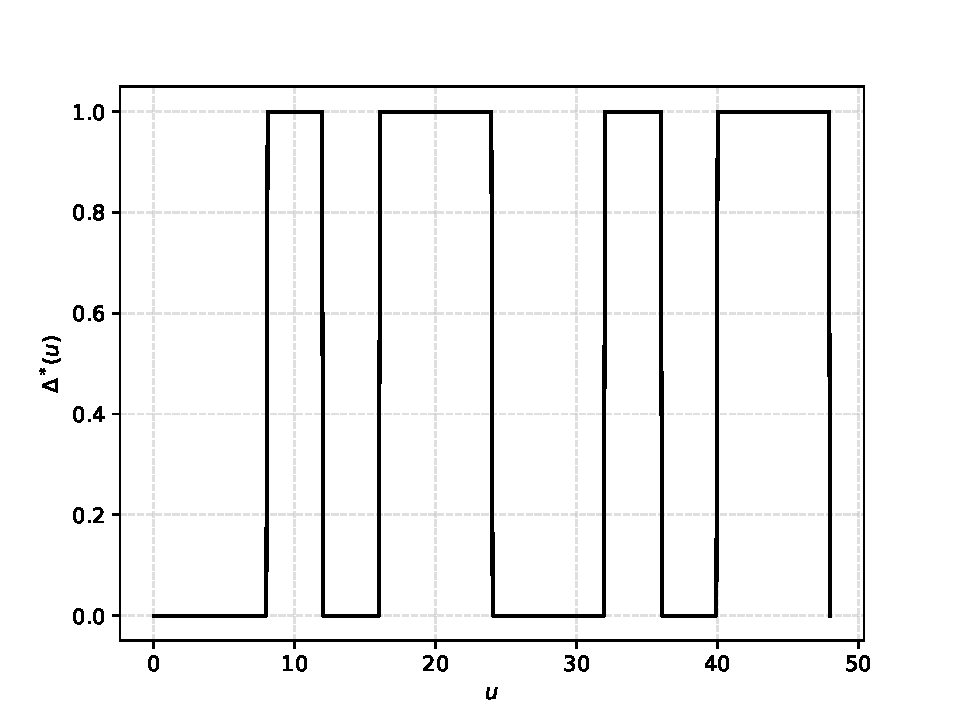
\includegraphics[width=\linewidth]{/home/tempdata/repos/thesis/static/misc/delta8m12q.pdf}
  \end{minipage}
  \hfill
  \begin{minipage}[t]{0.48\textwidth}
    \centering
    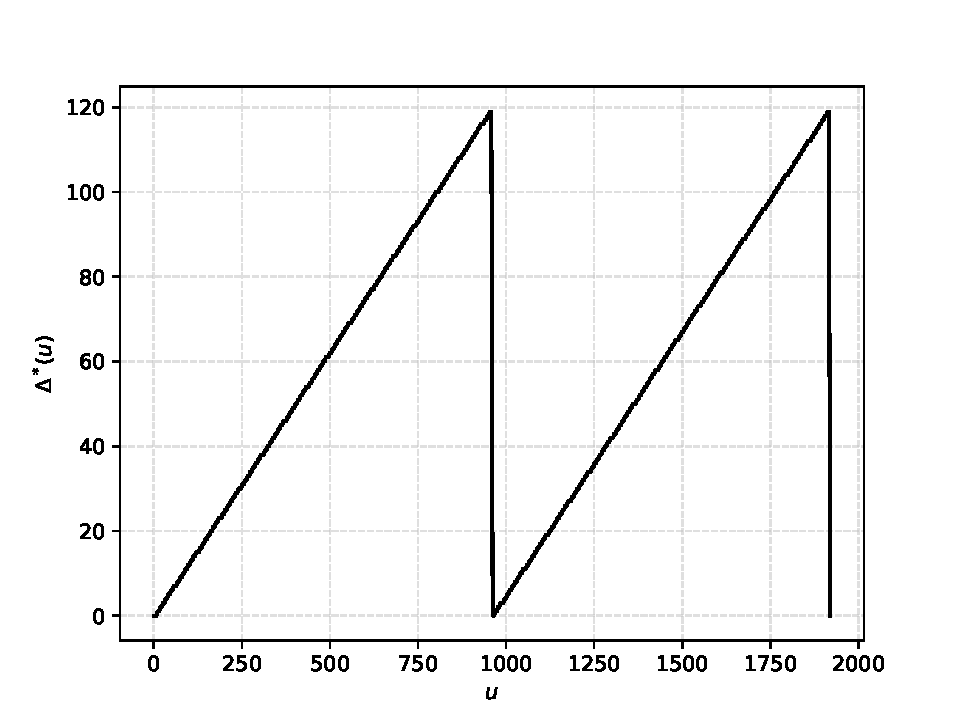
\includegraphics[width=\linewidth]{/home/tempdata/repos/thesis/static/misc/delta008m960q.pdf}
  \end{minipage}

  \caption{Número de capas a revisar en función del presupuesto. \textit{Izquierda: }Para los
	  parámetros $m = 8$ y $q^* = 12$ encontramos que hay un máximo de una capa a revisar.
	\textit{Derecha: } A medida que $m$ se vuelve fraccionario, las capas a revisar aumentan. En
		este caso tenemos $m = 0.08$ y $q^* = 960$.}
  \label{fig:m:ex}
\end{figure}

Observaremos en el análisis de resultados que el número de capas enteras que nuestro algoritmo
revisa en realidad disminuye a medida que aumenta el presupuesto $u$. Demostraremos a continuación
que para $u$ suficientemente grande, la solución al problema (\ref{theory:formulation}) se encuentra
en la $\eta$-ésima capa entera. Este resultado será análogo al Teorema \ref{infinite:th:complexity}.
No obstante, requerimos de un par de Definiciones y Lemas preliminares. Para motivar lo que
se encuentra a continuación mencionamos lo siguiente.

Primero mostramos que existe un punto entero en una vecindad fija de cada punto sobre cualquier capa
entera. Luego, si el entero $k$ que parametriza la capa entera es suficientemente grande, debe ser
el caso que existe una vecindad de un punto no negativo tal que esté completamente contenida en el
cuadrante no negativo. Como necesariamente hay un punto entero en esa vencidad, habremos de
encontrar un punto entero no negativo sobre esa $k$-ésima capa entera.

\begin{definition}
	\label{fin:def:ball}
	Sea $H_{\vec{q}, k\norm{\vec{q}}^{-2}}$ una capa entera. Entonces definimos la \textbf{bola
	cerrada} sobre
	esta capa entera con radio $r > 0$ y centro $\vec{x} \in H_{\vec{q}, k\norm{\vec{q}}^{-2}}$ como
	\begin{equation}
		\label{eq:k-ball}
		B_r^{(k)}(\vec{x}) \coloneq \lbrace \vec{y} \in \R^n \colon \norm{\vec{y} - \vec{x}} \leq r
		\rbrace \cap H_{\vec{q}, k \norm{\vec{q}}^{-2}}.
	\end{equation}
\end{definition}
% TODO: mostrar una imagen con una bola.
\begin{lemma}
	\label{lemma:ball-cover}
	Sea $\vec{q} \in \Z^n$ tal que sus entradas son coprimas y supongamos que $q_n \neq 0$. Entonces
	existe $r > 0$ tal que la familia de bolas
	\begin{equation*}
		\left\lbrace B_r^{(k)}(\vec{x}) \colon \vec{x} \in H_{\vec{q}, k\norm{\vec{q}}^{-2}} \cap
			\Z^n \right\rbrace
	\end{equation*}
	es una cubierta de la $k$-ésima capa entera $H_{\vec{q}, k\norm{\vec{q}}^{-2}}$.
\end{lemma}
\begin{proof}
	Como $q_n \neq 0$, recordemos del Teorema \eqref{th:lattice} que
	\begin{equation*}
		\vec{x} \in H_{\vec{q}, k\norm{\vec{q}}^{-2}} \cap \Z^n \iff \vec{x} = k\vec{\nu} + M\vec{t}
	\end{equation*}
	para algún vector $\vec{t} \in \Z^{n-1}$, donde recuperamos $\vec{\nu}$ y $M$ de
	\eqref{eq:vec-omega} y \eqref{eq:mat-T}, respectivamente. Así, tenemos
	\begin{equation*}
		\left\lbrace B_r^{(k)}(\vec{x}) \colon \vec{x} \in H_{\vec{q}, k\norm{\vec{q}}^{-2}} \cap
			\Z^n \right\rbrace
			=
		\left\lbrace B_r^{(k)}(k\vec{\nu} + M\vec{t}) \colon \vec{t} \in \Z^{n-1} \right\rbrace.
	\end{equation*}
	A partir de esto último sabemos que $B_r^{(k)}(k\vec{\nu} + M\vec{t}) \subseteq H_{\vec{q},
	k\norm{\vec{q}}^{-2}}$ para todo punto entero $\vec{t} \in \Z^{n-1}$. Luego, para cualquier $r >
	0$ tenemos
	\begin{equation}
		\label{eq:ball-cover:1}
		\bigcup_{\vec{t} \in \Z^{n-1}}B_r^{(k)}(k\vec{\nu} + M\vec{t}) \subseteq
		H_{\vec{q}, k\norm{\vec{q}}^{-2}}.
	\end{equation}
	Ahora bien, sea $\vec{y}$ un punto sobre la $k$-ésima capa entera. Por el Lema \ref{lemma:iso2}
	sabemos que las columnas de $M$ son linealmente independientes, y entonces existe $\vec{t} \in
	\R^{n-1}$ tal que
	\begin{equation*}
		\vec{y} = k\vec{\nu} + M\vec{t}.
	\end{equation*}
	Sea $\lfloor \vec{t} \rceil \in \Z^{n-1}$ el vector resultante de redondear cada entrada de
	$\vec{t}$ al entero más cercano. Luego, $\vec{t} = \lfloor \vec{t} \rceil + \vec{\delta}$,
	donde $\vec{\delta} \in \R^{n-1}$ satisface $\norm{\vec{\delta}}_{\infty} \leq 0.5$. Definamos
	\begin{equation*}
		\vec{x} \coloneq k\vec{\nu} + M\lfloor \vec{t} \rceil \in \Z^{n-1},
	\end{equation*}
	de donde se sigue que
	\begin{align}
		\norm{\vec{y} - \vec{x}}_2^{2} 
		&= \norm{M\vec{\delta}}_{2}^{2} \nonumber \\
		&\leq \sum_{i=1}^{n-1}|\vec{\delta}_i|^2 \norm{M\vec{e}_i}_2^{2} \nonumber \\
		&\leq \frac{1}{4}\sum_{i=1}^{n-1} \norm{M\vec{e}_i}_2^{2} \label{eq:alt-M-bound} \\
		&= \frac{1}{4}\norm{M}_F^2, \nonumber
	\end{align}
	donde $\norm{M}_F$ denota la norma Frobenius de $M$. Por lo tanto, si definimos
	\begin{equation}
		\label{eq:radius}
		r \coloneq \frac{1}{2}\norm{M}_F,
	\end{equation}
	encontramos que $\vec{y} \in B_r^{(k)}(\vec{x})$. Luego, como $\vec{y} \in H_{\vec{q},
	k\norm{\vec{q}}^2} \cap \Z^n$ fue genérico, se sigue que
	\begin{equation}
		\label{eq:ball-cover:2}
		H_{\vec{q}, k\norm{\vec{q}}^{-2}} \subseteq
		\bigcup_{\vec{t} \in \Z^{n-1}}B_r^{(k)}(k\vec{\nu} + M\vec{t}).
	\end{equation}
	Juntando esto con (\ref{eq:ball-cover:1}) obtenemos lo que queríamos demostrar.
\end{proof}

Ahora bien, denotemos por $\vec{u}_i$ las intersecciones que tiene la capa entera $H_{\vec{q},
k\norm{\vec{q}}^{-2}}$ con cada uno de los ejes. Es decir,
\begin{equation}
	\label{eq:generators}
	\vec{u}_i \coloneq \frac{k}{q_i}\vec{e}_i,
\end{equation}
y consideremos el símplice $\sigma$ generado por estos vectores:
\begin{equation*}
	\sigma \coloneq \left\lbrace \theta_1\vec{u}_1 + \cdots \theta_n\vec{u}_n \colon
		\sum_{i=1}^{n}\theta_i = 1, \theta_i \geq 0 \right\rbrace.
\end{equation*}
Se sigue inmediatamente que todo punto $\vec{x} \in \R^n$ no negativo sobre la $k$-ésima capa entera
también es un elemento de este símplice $\sigma$ y viceversa.

Ahora bien, nos interesa determinar la existencia de un punto entero sobre $\sigma$. De esta manera,
tendríamos un punto entero no negativo que satisface la ecuación lineal diofantina
$\vec{q}^T\vec{x} = k$. Para lograr esto, definimos el baricentro de $\sigma$ y determinamos una
vecindad de este baricentro de manera que esté contenida en el símplice.

\begin{definition}
	Dado un símplice $\sigma$ generado por $\vec{u}_1, \ldots, \vec{u}_n$, definimos su
	\textbf{baricentro} o \textbf{centro de masa} $\est{\sigma}$ como
	\begin{equation*}
		\est{\sigma} \coloneq \frac{1}{n} \sum_{i=1}^{n}\vec{u}_i.
	\end{equation*}
\end{definition}
\begin{observation}
	El baricentro $\est{\sigma}$ es un elemento de $\sigma$. Esto se debe a que $\est{\sigma}$ es la
	combinación convexa de $\vec{u}_1, \ldots, \vec{u}_n$, donde $\theta_1 = \cdots = \theta_n =
	\frac{1}{n}$.
\end{observation}

\begin{definition}
	Sea $\sigma$ un símplice y consideremos su baricentro $\est{\sigma}$. Definamos
	\begin{equation}
		\label{eq:def:r-sigma}
		r_\sigma \coloneq \max \lbrace r > 0 \colon B_r^{(k)}(\est{\sigma})
		\subseteq \sigma \rbrace.
	\end{equation}
	Entonces decimos que $\mathcal{C}^{(k)} \coloneq
	B_{r_\sigma}^{(k)}(\est{\sigma})$ es la \textbf{circunferencia inscrita} en $\sigma$. A
	$r_\sigma$ le llamamos el radio de tal circunferencia.
\end{definition}

\begin{definition}
	Sea $\sigma$ un símplice. Al símplice $F_j$ generado por los vectores $\lbrace \vec{u}_i
	\rbrace_{i \neq j}$ lo llamamos la \textbf{$j$-ésima faceta} de $\sigma$.
\end{definition}
\begin{observation}
	Si $\sigma$ es generado por $n$ vectores, entonces tiene $\binom{n}{n-1} = n$ facetas, y cada
	una es generada por $n - 1$ vectores. También se cumple que la frontera del símplice es la unión
	de sus facetas.
\end{observation}

De (\ref{eq:generators}) encontramos que el vector $\vec{u}_j$ es ortogonal a los vectores $\lbrace
\vec{u}_i \rbrace_{i \neq j}$, y por lo tanto su proyección sobre la capa entera $H_{\vec{q},
k\norm{\vec{q}}_2^{-2}}$ constituye el vector normal de la $j$-ésima faceta. Además, esta proyección
apunta hacia el interior del símplice $\sigma$. Como $\vec{q}$ es el vector normal a $H_{\vec{q},
k\norm{\vec{q}}_2}$, encontramos que la proyección de $\vec{u}_j$ sobre esta capa entera es
\begin{equation}
	\label{eq:normal-vector}
	\vec{\mu}_j \coloneq
	\vec{u}_j - \frac{\vec{q}^T\vec{u}_j}{\vec{q}^T\vec{q}}\vec{q}
	=
	\vec{u}_j - \frac{k}{\norm{\vec{q}}_2^2}\vec{q}.
\end{equation}
Denotemos por $\est{\mu}_j$ el vector $\vec{\mu}_j$ normalizado. Encontramos entonces que cada
faceta $F_j$ está contenida en el hiperplano afino
\begin{equation*}
	\lbrace \vec{x} \in \R^{n} \colon \est{\mu}_j^T\vec{x} = b_j \rbrace
	\cap H_{\vec{q}, k\norm{\vec{q}}_2^{-2}},
\end{equation*}
donde $b_j \coloneq \est{\mu}_j^T\vec{x}$ para algún $\vec{x} \in F_j$. Luego, como cada
vector normal $\est{\mu}_j$ apunta hacia el interior del símplice $\sigma$, se sigue que este puede
ser escrito como
\begin{equation*}
	\sigma = \bigcap_{j=1}^{n} \lbrace \vec{x} \in \R^{n} \colon \est{\mu}^T_j\vec{x} \geq b_j
	\rbrace \cap H_{\vec{q}, k\norm{\vec{q}}_2^{-2}}.
\end{equation*}
Esta caracterización de $\sigma$ nos permite demostrar el siguiente Lema.
\begin{lemma}
	\label{lemma:sigma-radius}
	El radio $r_\sigma$ de la circunferencia inscrita en $\sigma$ está dado por
	\begin{equation*}
		r_\sigma = \min_{1 \leq j \leq n} \lbrace d(\est{\sigma}, F_j) \rbrace,
	\end{equation*}
	donde $d(\est{\sigma}, F_j)$ denota la mínima distancia entre el baricentro
	$\est{\sigma}$ y la $j$-ésima faceta $F_j$ del símplice $\sigma$.
\end{lemma}
\begin{proof}
	Observemos que $\vec{u}_i$ con $i \neq j$ es un vector sobre el símplice $\sigma$. Luego, la
	distancia entre el baricentro y la $j$-ésima faceta es
	\begin{equation*}
		d(\est{\sigma}, F_j) = |\est{\mu}_j^T(\est{\sigma} - \vec{u}_i)|
		= \est{\mu}_j^T(\est{\sigma} - \vec{u}_i),
	\end{equation*}
	pues $\est{\sigma}$ es un elemento de $\sigma$ y $\est{\mu}_j$ apunta hacia adentro
	del símplice.

	Mostramos primero que si $r \leq \min_{1 \leq j \leq n} \lbrace d(\est{\sigma}, F_j) \rbrace$, entonces
	$B_r^{(k)}(\est{\sigma}) \subseteq \sigma$. Así pues, sea $\vec{x} \in
	B_r^{(k)}(\est{\sigma})$. Observemos que
	\begin{align*}
		\est{\mu}_j^T\vec{x} - b_j
		&=
		\est{\mu}_j^T(\vec{x} - \est{\sigma}) + \est{\mu}_j^T\est{\sigma} -
		b_j \\
		&= \est{\mu}_j^T(\vec{x} - \est{\sigma}) + d(\est{\sigma}, F_j).
	\end{align*}
	Por la desigualdad de Cauchy-Schwartz tenemos
	\begin{equation*}
		\est{\mu}_j^T(\vec{x} - \est{\sigma}) \geq -\norm{\est{\mu}_j}_2\norm{\vec{x} -
		\est{\sigma}}_2 = -\norm{\vec{x} - \est{\sigma}}_2 \geq -r,
	\end{equation*}
	y por lo tanto,
	\begin{equation*}
		\est{\mu}_j^T\vec{x} - b_j \geq -r + d(\est{\sigma}, F_j) \geq 0,
	\end{equation*}
	pues $r \leq d(\est{\sigma}, F_j)$ para todo $j \in \lbrace 1, \ldots, n \rbrace$. Así,
	encontramos que, para todo $\vec{x} \in B_r^{(k)}(\est{\sigma})$,
	\begin{equation*}
		\vec{x} \in
		\bigcap_{j=1}^{n} \lbrace \vec{x} \in \R^{n-1} \colon \est{\mu}^T_j\vec{x} \geq b_j \rbrace
		\cap H_{\vec{q}, k\norm{\vec{q}}_2^{-2}} = \sigma,
	\end{equation*}
	y por lo tanto $B_r^{(k)}(\est{\sigma}) \subseteq \sigma$. A causa de
	(\ref{eq:def:r-sigma}) encontramos que $r_\sigma \geq \min_{1 \leq j \leq n} \lbrace
	d(\est{\sigma}, F_j) \rbrace$.

	Ahora bien, supongamos que $r > d(\est{\sigma}, F_j)$ para algún $j \in \lbrace 1, \ldots,
	n \rbrace$. Consideremos el punto $\vec{x} \in F_j$ que satisface $d(\est{\sigma}, F_j) =
	d(\est{\sigma}, \vec{x})$. Tal punto existe porque $F_j$ es cerrado. Luego,
	$\norm{\est{\sigma} - \vec{x}}_2 < r$. Entonces existe $\varepsilon > 0$ tal que
	\begin{equation*}
		\norm{\est{\sigma} - (\vec{x} - \varepsilon\est{\mu}_j)}_2 \leq r,
	\end{equation*}
	lo que implica que $\vec{x} - \varepsilon\est{\mu}_j \in
	B_r^{(k)}(\est{\sigma})$. Sin embargo, tenemos
	\begin{equation*}
		\est{\mu}_j^T(\vec{x} - \varepsilon\est{\mu}_j) = b_j - \varepsilon\norm{\est{\mu}_j}_2^2 < b_j,
	\end{equation*}
	y entonces $\vec{x} - \varepsilon\est{\mu} \not\in \sigma$. De aquí se sigue que $r_\sigma
	\leq d(\est{\sigma}, F_j)$ para todo $j \in \lbrace 1, \ldots, n \rbrace$ y, por lo tanto,
	$r_\sigma \leq \min_{1 \leq j \leq n} \lbrace d(\est{\sigma}, F_j) \rbrace$.

	Concluimos, entonces, con
	\begin{equation*}
		r_\sigma = \min_{1 \leq j \leq n} \lbrace d(\est{\sigma}, F_j) \rbrace,
	\end{equation*}
	que es lo que queríamos demostrar.
\end{proof}

Buscamos expresar el radio $r_\sigma$ en función de $k$, por lo que debemos realizar un par de
cálculos. Retomemos de la demostración del Lema anterior que la distancia entre el baricentro y la
$j$-ésima faceta está dada por
\begin{equation*}
	d(\est{\sigma}, F_j) = \frac{{\vec{\mu}}_j^T(\est{\sigma} - \vec{\mu}_j)}{\norm{\vec{\mu}_j}_2}.
\end{equation*}
Realizando los cálculos, encontramos que
\begin{align*}
	\vec{\mu}_j^T(\est{\sigma} - \vec{u}_i)
	% &=
	% \left( \frac{k}{q_j}\vec{e}_j - \frac{k}{\norm{\vec{q}}_2^2}\vec{q} \right)^T
	% \left( \frac{k}{nq_1}, \ldots, \frac{k}{nq_i} - \frac{k}{q_i}, \ldots,
	% 		\frac{k}{nq_n} \right) \\
	% &=
	% k^2
	% \left( \frac{1}{q_j}\vec{e}_j - \frac{1}{\norm{\vec{q}}_2^2}\vec{q} \right)^T
	% \left( \frac{1}{nq_1}, \ldots, \frac{1}{nq_i} - \frac{1}{q_i}, \ldots,
	% 		\frac{1}{nq_n} \right) \\
	% &=
	% k^2
	% \left(\frac{1}{q_j}\frac{1}{nq_j} -
	% 	\frac{1}{\norm{\vec{q}}_2^2} \cdot
	% 	\left(\frac{1}{n} + \cdots + \frac{1}{n} - 1\right)
	% 	\right) \\
	&= \frac{k^2}{nq_j^2},
\end{align*}
y también
\begin{equation*}
	\norm{\vec{\mu}_j}_2 = k \sqrt{\frac{1}{q_j^2} - \frac{1}{\norm{\vec{q}}_2^2}}.
\end{equation*}
Sustituyendo valores, obtenemos
\begin{equation*}
	d(\est{\sigma}, F_j) = \frac{k}{n} \cdot
	\frac{1}{q_j^2\sqrt{q_j^{-2} - \norm{\vec{q}}_2^{-2}}}
	= \frac{k}{n} \cdot \frac{1}{Q_j},
\end{equation*}
donde definimos $Q_j$ pertinentemente. Finalmente, del Lema \ref{lemma:sigma-radius} encontramos que
el radio de la circunferencia inscrita en el símplice $\sigma$ está dado por
\begin{equation}
	\label{eq:sigma-radius}
	r_\sigma = \min_{1 \leq j \leq n} \lbrace d(\est{\sigma}, F_j) = \frac{k}{n} \cdot
	\frac{1}{\max_{1 \leq j \leq n} \lbrace Q_j \rbrace}
\end{equation}

\begin{theorem}
	\label{th:intsimplex}
	Existe un punto entero sobre el símplice $\sigma$ para $k$ suficientemente grande.
\end{theorem}
\begin{proof}
	Consideremos $r$ definida en (\ref{eq:radius}). Por el Lema \ref{lemma:ball-cover} sabemos que
	existe un punto entero $\vec{x}$ en $B_r^{(k)}(\est{\sigma})$. Como la circunferencia
	$\mathcal{C}^{(k)}$ está inscrita en $\sigma$, basta mostrar que existe $k$
	suficientemente grande tal que $r \leq r_\sigma$, pues esto implicaría
	\begin{equation*}
		\vec{x} \in B_r^{(k)}(\est{\sigma}) \subseteq \mathcal{C}^{(k)} \subseteq \sigma.
	\end{equation*}
	De (\ref{eq:sigma-radius}) obtenemos que $r \leq r_\sigma$ si y solo si
	\begin{equation}
		\label{eq:eta-limit}
		k \geq \frac{n}{2}\norm{M}_F\max_{1 \leq j \leq n} \lbrace Q_j \rbrace,
	\end{equation}
	que es lo que queríamos demostrar.
\end{proof}
De \eqref{eq:eta-limit} parece que podemos concluir que hay una dependencia lineal entre la
dimensión $n$ y el lado derecho $k$. No obstante, la norma $\norm{M}_F$ también depende
implícitamente de $n$. Para ser más explícitos con respecto a esta dependencia, podemos rescatar de
\eqref{eq:alt-M-bound} la siguiente cota:
\begin{equation*}
	\frac{1}{4}\sum_{i=1}^{n-1}\norm{M\vec{e}_i}_2^2
	\leq
	\frac{n-1}{4}\max_{1 \leq j \leq n} \lbrace \norm{M\vec{e}_j}_2^2 \rbrace,
\end{equation*}
de donde reemplazaríamos la cota \eqref{eq:eta-limit} en el Teorema \ref{th:intsimplex},
\begin{equation*}
	k \geq \frac{n\sqrt{n-1}}{2} \max_{1 \leq j \leq n} \lbrace \norm{M\vec{e}_j}_2 \rbrace \cdot
	\max_{1 \leq j \leq n} \lbrace Q_j \rbrace.
\end{equation*}
Esta cota, no obstante, es más grande que la propuesta inicialmente.

Además, el resultado que obtuvimos es más fuerte de lo que aparenta. Hemos encontrado una
cota inferior de manera que podamos asegurar la existencia de puntos enteros en una vecindad del
baricentro $\est{\sigma}$. Este punto no es especial, pues en realidad podemos realizar el mismo
procedimiento enfocándonos en otros puntos del símplice $\sigma$ para asegurar soluciones en sus
respectivas vecindades. Entonces, dependiendo del punto, podemos obtener mejores o peores cotas para
$k$. El punto más interesante es aquel que provee la cota inferior más pequeña\footnote{
	El autor tiene razones para sospechar que este punto se encuentra en la intersección de todos
	los vectores normales a cada faceta $F_j$.
}.

De manera inmediata obtenemos también los siguientes Teoremas. Cabe mencionar que estos resultados
solamente muestran la existencia de una solución entera $\vec{x}$ no negativa para la ecuación lineal
diofantina $\vec{q}^T\vec{x} = k$. Será en la Sección \ref{subsec:complex} que discutiremos cómo
encontrar esta solución.
\begin{theorem}
	\label{th:intnonneg1}
	Sea $\vec{q} \in \Z^n$ tal que sus entradas son coprimas y supongamos que $\vec{q} > \vec{0}$.
	Entonces la ecuación lineal diofantina $\vec{q}^T\vec{x} = k$ tiene soluciones enteras no
	negativas para $k$ suficientemente grande.
\end{theorem}
\begin{proof}
	Consideremos el símplice $\sigma$ generado por los vectores \eqref{eq:generators} y supongamos
	que $k$ satisface la cota en \eqref{eq:eta-limit}. Por el Teorema \ref{th:intsimplex}, se sigue
	que $\sigma$ contiene un punto entero $\vec{x}$ y, por lo tanto, $\vec{x}$ también es no
	negativo. Pero $\sigma$ está contenida en la $k$-ésima capa entera, lo que implica que $\vec{x}
	\in H_{\vec{q}, k\norm{\vec{q}}^{-2}}$ y entonces, por el Lema \ref{theory:lemma:utility},
	$\vec{x}$ satisface la ecuación lineal diofantina $\vec{q}^T\vec{x} = k$.
\end{proof}
\begin{theorem}
	Sea $\vec{p} \in \R^n$ un vector esencialmente entero y supongamos que su múltiplo coprimo
	$\vec{q}$ tiene entradas estrictamente positivas. Entonces el problema
	\eqref{theory:formulation} se puede resolver a través de encontrar la solución de una sola
	ecuación lineal en $n$ incógnitas para un presupuesto $u$ suficientemente grande.
\end{theorem}
\begin{proof}
	Por la Definición \ref{theory:def:rational} sabemos que existe un escalar $m \in \R$ tal que
	$\vec{p} = m\vec{q}$. Supongamos, sin pérdida de generalidad, que $m$ es positivo. Del Lema
	\ref{phase-1:lemma:eta} tenemos que el entero $\eta$ parametriza la primera capa entera en
	satisfacer el presupuesto y que $\eta = \floor{u/m}$. Por el Teorema \ref{th:intnonneg1} sabemos
	que si $\eta$ es suficientemente grande, entonces la ecuación lineal diofantina
	$\vec{q}^T\vec{x} = \eta$ tiene al menos una solución entera no negativa $\vec{x}$. Luego,
	$\vec{x}$ es factible para el problema \eqref{theory:formulation}, pero por la maximalidad de
	$\eta$ encontramos que $\vec{x}$ también es un punto óptimo. En conclusión, solo deviene
	necesario resolver una ecuación lineal diofantina para determinar la solución del problema
	\eqref{theory:formulation}.
\end{proof}

El Teorema \ref{th:intnonneg1} junto con la cota \eqref{eq:eta-limit} provee, hasta donde llega el
conocimiento del autor, nuevas cotas superiores para los números de Frobenius\footnote{
	Véase el Problema de la Moneda en \url{https://en.wikipedia.org/wiki/Coin_problem}.
}. De manera resumida,
dada una colección de enteros $a_1, \ldots, a_n$ coprimos, el número de Frobenius es el entero $F$
más grande tal que $F$ no pueda ser expresado como una combinación lineal entera no negativa de
$a_1, \ldots, a_n$. Un estudio sobre cómo se compara esta colección de cotas con respecto a la
literatura existente, si bien interesante, queda fuera del propósito de esta tesis.

En último lugar, mencionamos que eventualmente es suficiente con revisar la primera capa entera. No
hemos demostrado, empero, que el número de capas enteras a revisar eventualmente decrece en cuanto
$u$ aumenta. Observaremos en el análisis de resultados que hay un patrón periódico y decreciente en
cuanto al número de capas enteras revisadas. Demostrar, en cambio, que este comportamiento siempre
se cumple es mucho más difícil y queda fuera del propósito de esta tesis.

\section{Construcción de soluciones}
\label{subsec:complex}

\noindent
Sea $\vec{p} \in \R^n$ un vector esencialmente entero y supongamos que las entradas de su múltiplo
coprimo $\vec{q}$ son todas estrictamente positivas. Supongamos, sin pérdida de generalidad, que el
escalar $m$ que satisface $\vec{p} = m\vec{q}$ es también positivo. Bastante hemos discutido sobre
cómo la solución del problema \eqref{theory:formulation} se traduce a la búsqueda de una solución
entera no negativa de la ecuación lineal diofantina $\vec{q}^T\vec{x} = k$ para alguna $k \leq \eta$,
donde $\eta$ es tomada del Lema \ref{phase-1:lemma:eta}.

En la primera parte de esta sección presentamos los algoritmos \ref{algo:fin:helper} y
\ref{algo:fin:dioph}, los cuales se encargan de obtener estas soluciones enteras no negativas que
tanto buscamos y, consecuentemente, también se encargan de resolver el problema original
\eqref{theory:formulation}.

% En la segunda parte de esta sección discutimos de manera un tanto informal la complejidad
% algorítmica del Algoritmo \ref{algo:fin:dioph}. Por lo tanto, también discutimos, así como lo
% hicimos en el capítulo \ref{chap:inf}, sobre la complejidad del problema \eqref{theory:formulation}
% en el caso especial de que $\vec{q} > \vec{0}$.

\begin{theorem}
	\label{th:fin:helper:correct}
	El algoritmo \ref{algo:fin:helper} es correcto.
\end{theorem}
\begin{proof}
	Hacemos la demostración por inducción en la dimensión $n$ del vector $\vec{q}$. Supongamos, para
	el caso base, que $n = 2$. Luego, queremos encontrar soluciones enteras no negativas de la
	ecuación
	\begin{equation}
		\label{lemma:correct:base-case}
		q_1x_1 + q_2x_2 = k.
	\end{equation}
	Por hipótesis sabemos que $q_1$ y $q_2$ son coprimos. Luego, del Teorema
	\ref{prerreq:th:construction}, las soluciones enteras de esta ecuación están dadas por
	\begin{equation}
		\label{lemma:correct:base-case:sol}
		\begin{cases}
			x_1 = kx_1' + q_2t, \\
			x_2 = kx_2' - q_1t, \\
		\end{cases}
	\end{equation}
	donde $t \in \Z$ es una variable libre, y $x_1', x_2'$ son los coeficientes de Bézout (c.f.
	Definición \ref{prerreq:def:bezout}) de $x_1, x_2$. Por claridad, escribimos $x_1'$ y $x_2'$
	como $x_{n-1}'$ y $x_{n}'$ en la línea \eqref{alg:fin:bez}. Despejando de estas soluciones,
	encontramos que existen soluciones no negativas si y solo si existe $t \in \Z$ que satisfaga
	\begin{equation*}
		\ceil{-\frac{kx_1'}{q_2}} \leq t \leq \floor{\frac{kx_2'}{q_1}}.
	\end{equation*}
	Los enteros $b_1$ y $b_2$ en las líneas \eqref{alg:fin:b1} y \eqref{alg:fin:b2} representan el
	lado izquierdo y derecho de estas desigualdades, respectivamente. De esta manera, el algoritmo
	devuelve \NIL~ si solo si este intervalo no está bien definido, es decir, si y solo si no existen
	soluciones enteras no negativas. Supongamos, pues, que este intervalo sí está bien definido.
	Entonces, podemos escoger que la variable libre $t$ sea $b_1$. Sustituyendo en
	\eqref{lemma:correct:base-case:sol} obtenemos una solución entera no negativa a la ecuación
	\eqref{lemma:correct:base-case} (líneas \eqref{alg:fin:xprev} y \eqref{alg:fin:xlast}) y entonces
	el algoritmo es correcto para $n = 2$.

	Supongamos, inductivamente, que el algoritmo es correcto para alguna $n - 1 \geq 2$. Mostramos
	ahora que el algoritmo también es correcto para $n$. Entonces deseamos encontrar soluciones
	enteras no negativas de la ecuación \eqref{eq:dioph} Haciendo la misma sustitución que en
	\eqref{eq:dioph:first-step}, recordando que $q_1, \ldots, q_n$ son coprimos por hipótesis, que
	definimos $\omega_1 \coloneq k$, y renombrando las variables ($x$ en vez de $x_1$, $g$ en vez de
	$g_2$ y $\omega$ en vez de $\omega_2$), obtenemos la ecuación
	\begin{equation}
		\label{lemma:correct:eq}
		q_1x + g\omega = k.
	\end{equation}
	Observemos que, como $g_1 = 1$, el entero $g = \gcd{q_2/g_1, \ldots, q_n/g_1}$, es equivalente a
	lo que se encuentra en la línea \eqref{alg:fin:g}. Por el Teorema \ref{prerreq:th:construction}
	tenemos que las soluciones enteras están dadas por
	\begin{equation}
		\label{lemma:correct:sol}
		\begin{cases}
			x = kx' + gt, \\
			\omega = k\omega' - q_1t,
		\end{cases}
	\end{equation}
	donde $t \in \Z$ es una variable libre, y $x', \omega'$ son los coeficientes de Bézout de $x,
	\omega$. Recordemos de \eqref{eq:dioph:first-step} que
	\begin{equation}
		\label{lemma:correct:eq-omega}
		\omega = \frac{q_2}{g}x_2 + \ldots + \frac{q_n}{g}x_n.
	\end{equation}
	Como $\vec{q} > \vec{0}$ por hipótesis, $g > 0$ porque el máximo común divisor siempre es
	positivo, y exigimos que $x_2, \ldots, x_n$ sean no negativos, debe ser el caso que $\omega$
	también sea no negativo. Luego, despejando de \ref{lemma:correct:sol}, existen soluciones no
	negativas de la ecuación \eqref{lemma:correct:eq} si y solo si existe $t \in \Z$ que satisfaga
	\begin{equation*}
		\ceil{-\frac{kx'}{g}} \leq t \leq \floor{\frac{k\omega'}{q_1}}.
	\end{equation*}
	Los enteros $b_1$ y $b_2$ en las líneas \eqref{alg:fin:b11} y \eqref{alg:fin:b21} representan el
	lado izquierdo y derecho de estas desigualdades, respectivamente. Si no existe tal variable
	libre $t \in \Z$ es porque el intervalo $[b_1, b_2]$ no está bien definido y por lo tanto $b_2 <
	b_1$. El algoritmo entonces salta a la línea \eqref{alg:fin:return} y devuelve \NIL.

	Si el intervalo $[b_1, b_2]$ está bien definido, podemos asegurar la no negatividad de $x$ en
	\eqref{lemma:correct:sol} para cualquier elección de $t$ en $[b_1, b_2$] y en
	la línea \eqref{alg:fin:subeq} nos encargamos entonces de encontrar soluciones enteras no negativas
	de la ecuación \eqref{lemma:correct:eq-omega}. Se verifica automáticamente que los coeficientes
	del lado derecho de esta ecuación son coprimos y constituyen justamente las entradas del vector
	$\vec{q}^{\texttt{tail}}$ (c.f. línea \eqref{alg:fin:qt}). Como $g > 0$ se sigue que
	$\vec{q}^{\texttt{tail}} > \vec{0}$. Luego, $\vec{q}^{\texttt{tail}}$ satisface las hipótesis
	del algoritmo.

	Por hipótesis inductiva, tenemos o bien que $\vec{x}^{\texttt{tail}}$ es entero no negativo y
	solución de \eqref{lemma:correct:eq-omega}, o bien es \NIL. En el primer caso y definiendo
	$\vec{x}$ como el vector de la línea \eqref{alg:fin:vecx} encontramos que
	\begin{equation*}
		\vec{q}^T\vec{x} = q_1x + g\left(\vec{q}^{\texttt{tail}}\right)^T\vec{x}^{\texttt{tail}}
		= q_1x + g\omega = k.
	\end{equation*}
	Pero $x \geq 0$ por construcción y $\vec{x}^{\texttt{tail}} \geq \vec{0}$ por este caso de la
	hipótesis inductiva. Así, $\vec{x}$ también es no negativo.

	Finalmente, en caso de que $\vec{x}^{\texttt{tail}}$ sea \NIL, iteramos sobre otra elección de
	la variable libre $t$ y regresamos al caso pasado. En caso de que este vector sea \NIL~ para
	todas las elecciones posibles de $t$ en el intervalo de factiblidad $[b_1, b_2]$, se sigue por
	hipótesis inductiva que la ecuación \eqref{lemma:correct:eq-omega} no tiene solución entera no
	negativa y por lo tanto tampoco la tiene la ecuación \eqref{eq:dioph}. Una vez agotadas estas
	elecciones finitas, devolvemos \NIL~ en la línea \eqref{alg:fin:return}.

	En conclusión, si el algoritmo es correcto para vectores $\vec{q}$ con dimensión $n - 1 \geq 2$,
	entonces también es correcto para vectores $\vec{q}$ con dimensión $n$. Juntando esto con el
	caso base, se sigue por inducción que el algoritmo es correcto para toda $n \geq 2$, que es lo
	que queríamos demostrar.
\end{proof}

Observemos que la elección del parámetro libre $t$ en el intervalo de factiblidad $I$ definido en la
línea \eqref{alg:fin:feas} del Algoritmo \ref{algo:fin:helper} es similar a la elección del
subproblema $S_i$ de optimización definido en la línea \eqref{p1c9:alg:BB_loop} del Algoritmo
\ref{algo:bb}. La diferencia radica en que, como todos los puntos enteros sobre la $k$-ésima capa
entera tienen el mismo nivel de utilidad $k$, no es necesario desarrollar políticas de poda así como
lo hicimos en el Ejemplo \ref{ex:ilp} en la Sección \ref{sec:prerreq}. De cierta manera, la única
política de poda posible es la de infactibilidad por no respetar la no negatividad de un punto
entero. Discutiremos más sobre esto cuando introduzcamos múltiples restricciones al problema
\eqref{theory:formulation}.

\begin{theorem}
	\label{th:fin:dioph:correct}
	El algoritmo \ref{algo:fin:dioph} es correcto.
\end{theorem}
\begin{proof}
	A causa del Teorema \ref{th:fin:helper:correct} basta verificar que el algoritmo termina y no
	devuelve \NIL. Además, obtenemos la maximalidad de $k$ debido a la manera en la que iniciamos el
	ciclo en la línea \eqref{alg:fin:loop}. Tenemos $0 \leq \eta$ por hipótesis y observemos que
	$\vec{0}$ es la única solución entera no negativa de la ecuación lineal diofantina
	$\vec{q}^T\vec{x} = 0$. De esta manera, si la ecuación $\vec{q}^T\vec{x} = k$ no tiene solución
	para $0 < k \leq \eta$, entonces el algoritmo devuelve $\vec{0}$ debido al Teorema
	\ref{th:fin:helper:correct}.
\end{proof}

Sabemos, en realidad, por el Lema \ref{lemma:tau} que el parámetro $k$ definido en la línea
\eqref{alg:fin:loop} descenderá hasta 0 si y solo si el parámetro $\tau$ definido en \eqref{eq:tau}
es nulo. No obstante, la demostración del Teorema \ref{th:fin:dioph:correct} deviene más simple
cuando en el Algoritmo \ref{algo:fin:dioph} dejamos que $k$ se encuentre en $[0, \eta]$ en vez de
$[\tau, \eta]$. Esta modificación, sin embargo, no afecta en lo más mínimo la correctud o la
complejidad del algoritmo.

Siguiendo la misma directriz, vale la pena mencionar lo siguiente con respecto al Algoritmo
\ref{algo:fin:helper}. Varios lenguajes de programación, tales como Python, cuentan con un límite en
las llamadas de recursión que el usuario puede realizar\footnote{
	En la computadora del autor, por ejemplo, el valor predeterminado de este límite es 3000, y por
	lo tanto, solamente podría el autor resolver problemas con dimensión $n \leq 3000$.
}. Si bien este límite puede modificarse, aumenta la posibilidad de encontranos con un
desbordamiento de pila, pues este algoritmo no está expresado en forma de recursión
terminal\footnote{
	Véase \url{https://en.wikipedia.org/wiki/Tail_call}.
}.

Además, este algoritmo, por ejemplo, no minimiza el número de llamadas para calcular el máximo común
divisor en la línea \eqref{alg:fin:g}. En efecto, supongamos que un intervalo de factibilidad $I$
definido en la línea \eqref{alg:fin:feas} induce a que $\vec{x}^{\texttt{tail}}$ sea \NIL~ para todo
$t \in I$. Entonces estaríamos haciendo $|I|$ llamadas a \texttt{NonNegativeIntSol} en la línea
\eqref{alg:fin:subeq} con el mismo vector $\vec{q}^{\texttt{tail}}$ y, por lo tanto, estaríamos
calculando $|I|$ veces la misma $g$ en la línea \eqref{alg:fin:g}. Lo mismo ocurre con el cálculo de
los coeficientes de Bézout $x'$ y $\omega'$ en la línea \eqref{alg:fin:bez2}.

A pesar de los puntos anteriores, el autor decidió escribir el Algoritmo \ref{algo:fin:helper} de
esa manera debido a que se simplificaba de manera significativa la demostración del Teorema
\ref{th:fin:helper:correct}. Sin embargo, el autor realizó una implementación equivalente más
eficiente a través de ciclos para obtener los resultados de la siguiente sección.

\begin{algorithm}[ht]
	\LinesNumbered
	\SetKwProg{Fn}{Fn}{\string:}{}
	\SetKwFunction{Bezout}{Bezout}
	\SetKwFunction{length}{length}
	\SetKwFunction{NonNegativeIntSol}{NonNegativeIntSol}
	\Fn{\NonNegativeIntSol{$\vec{q}$, $k$}}{
		\KwData{\\
			Vector coprimo $\vec{q} > \vec{0}$ tal que \length{$\vec{q}$} $\geq 2$. \\
			Lado derecho $k \geq 0$.
			}
		\KwResult{\\
			Solución entera no negativa $\vec{x}$ a la ecuación lineal diofantina $\vec{q}^T\vec{x} =
			k$ o \NIL.
		}
		\Begin{
			$n \leftarrow$ \length{$\vec{q}$}\;
			\If{$n = 2$}{
				$x_{n-1}', x_n' \leftarrow$ \Bezout{$q_1$, $q_2$}\; \label{alg:fin:bez}
				$b_1 \leftarrow \ceil{-k x_{n-1}' / q_2}$\; \label{alg:fin:b1}
				$b_2 \leftarrow \floor{k x_{n}' / q_1}$\; \label{alg:fin:b2}

				\If{$b_2 < b_1$}{
					\Return $\NIL$\;
				}

				$x_{n-1} \leftarrow k x_{n-1}' + b_1q_2$\; \label{alg:fin:xprev}
				$x_{n} \leftarrow k x_{n}' - b_1q_1$\; \label{alg:fin:xlast}
				\Return{$(x_{n-1}, x_n)$}\;
			}

			$g \leftarrow \gcd{q_2, \ldots, q_n}$\; \label{alg:fin:g}
			$x', \omega' \leftarrow$ \Bezout{$q_1$, $g$}\; \label{alg:fin:bez2}
			$b_1 \leftarrow \ceil{-k x' / g}$\; \label{alg:fin:b11}
			$b_2 \leftarrow \floor{k \omega' / q_1}$\; \label{alg:fin:b21}
			$I \leftarrow \braces{b_1, b_1 + 1, \ldots, b_2}$\; \label{alg:fin:feas}

			$\vec{q}^{\texttt{tail}} \leftarrow (q_{i + 1} / g \vcentcolon 1 \leq i \leq n - 1)$\;
			\label{alg:fin:qt}
			\While{$I \neq \emptyset$}{
				elegir $t \in I$\;
				$\omega \leftarrow k\omega' - tq_1$\;
				$\vec{x}^{\texttt{tail}} \leftarrow$ \NonNegativeIntSol{$\vec{q}^{\texttt{tail}}$,
				$\omega$}\; \label{alg:fin:subeq}

				\If{$\vec{x}^{\texttt{tail}} \neq$ \NIL}{
					$r \leftarrow$ \length{$\vec{x}^{\texttt{tail}}$}\;
					$x \leftarrow k x' + tg$\; \label{alg:fin:x}
					\Return{$(x, x^{\texttt{tail}}_1, \ldots, x^{\texttt{tail}}_r$})\;
					\label{alg:fin:vecx}
				}

				$I \leftarrow I \setminus \braces{t}$\;
			}

			\Return $\NIL$\; \label{alg:fin:return}
		}
	}
	\caption{Algoritmo para obtener soluciones enteras no negativas a la ecuación lineal diofantina
	$\vec{q}^T\vec{x} = k$, dados ciertos supuestos sobre $\vec{q}$.}
	\label{algo:fin:helper}
\end{algorithm}
\begin{algorithm}[ht]
	\LinesNumbered
	\SetKwProg{Fn}{Fn}{\string:}{}
	\SetKwFunction{Bezout}{Bezout}
	\SetKwFunction{length}{length}
	\SetKwFunction{NonNegativeIntSol}{NonNegativeIntSol}
	\SetKwFunction{Dioph}{Dioph}
	\Fn{\Dioph{$\vec{q}$, $\eta$}}{
		\KwData{\\
			Vector coprimo $\vec{q} > \vec{0}$ tal que \length{$\vec{q}$} $\geq 2$. \\
			Lado derecho $\eta \geq 0$.
			}
		\KwResult{\\
			Solución entera no negativa $\vec{x}$ a la ecuación lineal diofantina $\vec{q}^T\vec{x}
			= k$ para algún $k \leq \eta$ con $k$ maximal.
		}
		\Begin{
			\For{$k \leftarrow \eta$ \KwTo $0$}{ \label{alg:fin:loop}
				$\vec{x} \leftarrow$ \NonNegativeIntSol{$\vec{q}$, $k$}\;
				\If{$\vec{x} \neq$ \NIL}{
					\Return{$\vec{x}$}\;
				}
			}
		}
	}
	\caption{Algoritmo para obtener soluciones enteras no negativas a la ecuación lineal diofantina
	$\vec{q}^T\vec{x} = \eta$, dados ciertos supuestos sobre $\vec{q}$.}
	\label{algo:fin:dioph}
\end{algorithm}
% Con respecto a la complejidad algorítmica de analizar capas enteras podemos decir lo siguiente.
% Supongamos que deseamos encontrar todas las soluciones de (\ref{theory:formulation}). Definamos
% \begin{equation}
% 	\label{phase-1:def:feasible-layer}
% 	P_k \coloneq H_{\vec{q}, k\norm{\vec{q}}^{-2}} \cap \Z_{\geq \vec{0}}^n
% 	=
% 	\lbrace \vec{x} \in \Z^n \vcentcolon \vec{q}^T\vec{x} = k, \vec{x} \geq \vec{0}
% 	\rbrace,
% \end{equation}
% y sea $T(n)$ el tiempo requerido para encontrar todos los puntos en $P_k$ o determinar que este
% conjunto es vacío. Es razonable suponer que $T(n)$ es exponencial en $n$. En efecto, cada par
% $(x_i, \omega_{i + 1})$ genera un intervalo de factibilidad $[t_i^{\min},
% t_i^{\max}]$. Este intervalo ciertamente depende de las elecciones previas de $t_1, \ldots,
% t_{i - 1}$, aunque suprimimos esta dependencia en la notación para tener mayor claridad. Para
% encontrar todos los puntos en $P_k$, el algoritmo recorre todas las posibilidades:
% \begin{equation}
% 	\label{phase-1:complexity:bounds}
% 	\prod_{i=1}^{\kappa_1} \min_{t_1, \ldots, t_{i-1}} \lbrace t_i^{\max} -
% 	t_i^{\min} \rbrace
% 	\leq T(n) \leq
% 	\prod_{i=1}^{\kappa_2} \max_{t_1, \ldots, t_{i-1}} \lbrace t_i^{\max} -
% 	t_i^{\min} \rbrace,
% \end{equation}
% donde $1 \leq \kappa_1 \leq n$ es el entero más grande que asegura que  $\min_{t_1, \ldots,
% t_{i - 1}}\lbrace t_i^{\max} - t_i^{\min} \rbrace$ sea positivo para todo $i \in
% \lbrace 1, \ldots, \kappa_1 \rbrace$. Definimos $\kappa_2$ de manera análoga. Se cumple que
% $\kappa_1 \leq \kappa_2$. Sean $\ell_{\min}, \ell_{\max}$ las longitudes del intervalo de
% factibilidad más pequeño y del más grande en todos los niveles, respectivamente. Es decir, definimos
% \begin{align}
% 	\ell_{\min} &\coloneq \min_{1 \leq i \leq \kappa_1} \left\lbrace \min_{t_1, \ldots,
% 	t_{i - 1}} \lbrace t_i^{\max} - t_i^{\min} \rbrace \right\rbrace,
% 	\\
% 			\ell_{\max} &\coloneq \max_{1 \leq i \leq \kappa_2} \left\lbrace \max_{t_1,
% 			\ldots, t_{i - 1}} \lbrace t_i^{\max} - t_i^{\max} \rbrace
% 		\right\rbrace.
% \end{align}
% Si $P_k$ es vacío, se sigue que no existe ningún intervalo factible en el nivel $n$, lo que implica
% que $\kappa_2 < n$. En caso contrario, el algoritmo recorre hasta el último nivel, por lo que $\kappa_1
% = \kappa_2 = n$. De (\ref{phase-1:complexity:bounds}), obtenemos
% \begin{equation}
% 	\ell_{\min}^{n} \leq T(n) \leq \ell_{\max}^{n}.
% \end{equation}
% En el peor de los casos, nuestro algoritmo recorre todas las capas enteras parametrizadas por
% $\lbrace k, k - 1, \ldots, \tau\rbrace$. Se sigue que
% \begin{align}
% 	\label{phase-1:time}
% 	\text{Tiempo de ejecución}
% 	= \mathcal{O}((k - \tau) \cdot T(n))
% 	= \mathcal{O}(c^{n}),
% \end{align}
% para alguna $c > 1$.
% 
% Ahora bien, este razonamiento aplica a la modificación de nuestro objetivo en donde decidimos buscar
% todas las soluciones posibles. En realidad solo nos interesa encontrar un punto óptimo, por lo que
% podemos concluir que una cota superior para la complejidad de nuestro algoritmo es
% (\ref{phase-1:time}). Asímismo, en la práctica encontramos que la diferencia $k - \tau$ es crucial
% para determinar cuántas capas enteras recorre nuestro algoritmo en el peor de los casos.
% 
% Hemos mostrado anteriormente que para $u$ suficientemente grande es suficiente con recorrer una
% capa. En caso de que $u$ no sea suficientemente grande, observaremos en el análisis de resultados
% cómo se distribuye el número de capas enteras que en realidad se visitan.

\section{Análisis de resultados}

\section{Aplicaciones}
